\chapter{X-Ray Computed Tomography}
\label{sec:ct}
While this thesis is primarily focused on noise reduction using \acrshort{gan}s, a brief overview of some of the basic principles behind \acrfull{ct} imaging will be given in this chapter. The focus will be on explaining the underlying theoretical foundation of \acrshort{ct} imaging, including the main sources of noise. An overview of common reconstruction methods, as well a more novel one, will also be presented.

\section{Theoretical Foundation}
\label{sec:ct:theoreticalfoundation}
X-ray \acrshort{ct} imaging is based on interaction between X-rays and matter. This interaction will attenuate X-rays that propagate through a sample according to the Beer-Lambert law, which is given as \cite{doi:10.1063/1.4950807}
\begin{equation}
    \label{eq:beerlambert}
    I = I_0 \rm{e}^{-\int_{l_0}^{l}\mu\left(x,y,E\right)dl},
\end{equation}
where $I_0$ and $I$ is the incident and the attenuated X-ray beam intensities at positions $l_0$ and $l$ respectively, and $\mu$ is the attenuation coefficient of the traversed matter. The integral in the exponent is the path of the beam through the sample. The attenuation coefficient is dependent on energy ($E$), and typical X-ray \acrshort{ct} systems span a range of wavelengths (i.e. energies). 
Because of this, \cref{eq:beerlambert} must be modified to also account for the polychromatic nature of the X-ray source. 

The total incident radiation can be determined by integrating over all photon energies, 
\begin{equation}
    \label{eq:incidentradiation}
    I_0 = \int_{E_{min}}^{E_{max}}N\left(V,I\right)S\left(E\right)D\left(E\right)dE,
\end{equation}
with $N\left(V,I\right)$ being a variable introduced to account for photon flux depending on X-ray source tube voltage $V$ and current $I$, $S\left(E\right)$ being the normalized X-ray source spectrum modulated by the absorption materials between the source and the detector (not including the sample), and $D\left(E\right)$ being the detector sensitivity modulated by protection materials on the detector. $E_{min}$ and $E_{max}$ bound the energy range of the radiation spectrum. 

By combining \cref{eq:beerlambert,eq:incidentradiation}, we get the modified Beer-Lambert law accounting for the polychromatic X-rays \cite{doi:10.1063/1.4950807}, 
\begin{equation}
    I = \int_{E_{min}}^{E_{max}}N\left(V,I\right)S\left(E\right)D\left(E\right)\rm{e}^{-\int_{l_0}^{l}\mu\left(x,y,E\right)dl}dE.
\end{equation}
This can be solved for the attenuation coefficient projection, giving \cite{doi:10.1063/1.4950807}
\begin{equation}
    \label{eq:ctattenuationcoefficient}
    \int_{l_0}^{l} \mu_m\left(x,y\right)dl = -\ln\left[\frac{\int S\left(E\right) D\left(E\right)\rm{e}^{-\int_{l_0}^{l}\mu\left(x,y,E\right)dl} dE }{ \int S\left(E\right) D\left(E\right) dE }\right].
\end{equation}
The attenuated radiation $I_0$ can be related to the attenuation coefficient projection $\mu_m$ of a path through the sample by use of this equation. When the attenuation coefficient projections are known, the sample itself can be reconstructed using a reconstruction algorithm if a sufficient number of projections are available. 

\subsection{Noise}
Assuming a sufficient number of projections of the attenuation coefficient are available, the primary sources of noise in \acrshort{ct} measurements are quantum noise and electronic noise \cite{boas2012ct}. 

The quantum noise, sometimes also known as shot noise or simply Poisson noise, is due to the statistical error of low photon counts. It can be modeled as a Poisson distribution \cite{Whiting2006},
\begin{equation}
    \label{eq:poissonnoise}
    P(X = x) = \frac{\rm{e}^{-xm}m^x}{x!},
\end{equation}
with $m$ being the mean signal value, $x=0,1,...$ being an integer representing the measured signal value, and $X$ being a random variable denoting the number of photons generated by the X-ray source. Quantum noise can be reduced simply by increasing the incident X-ray beam intensity, however this is often not wanted as increasing the radiation dose has raised conserns about potential health risks \cite{doi:10.1056/NEJMra072149,PEARCE2012499}. 

Electronic noise is related to the electronics of the X-ray detector, and it is modeled as additive white Gaussian (i.e. normal) noise \cite{boas2012ct},
\begin{equation}
    \mathcal{N}\left(0,\sigma \right) = \frac{1}{2\pi\sigma}\rm{e}^{-\frac{x^2}{2\sigma}},
\end{equation}
which corresponds to a normal distribution $\mathcal{N}\left(\mu,\sigma\right)$ with mean signal value $\mu=0$ and standard deviation $\sigma$. 

If an insufficient number of projections of the attenuation coefficient are available, it is known as a missing wedge problem. Missing wedge measurements are incomplete datasets with respect to standard requirements of established reconstruction algorithms \cite{10.1111/jmi.12313}. This leads to noise artefacts that appear as elongations of reconstructed details along the mean direction (i.e. the symmetry centre of the projections). Several different methods of reducing this artefacting have been tried, including different reconstruction algorithms \cite{10.1111/jmi.12313} and \acrshort{ml} based approaches \cite{liu2020tomogan}. Missing wedge artefacting will be refered to as noise in this thesis. 

A comparison of quantum noise and missing wedge artefacting on a dataset imaging glass beads can be seen in \cref{fig:noisecomparison}. 

\begin{figure}[htbp]  
    \centering
    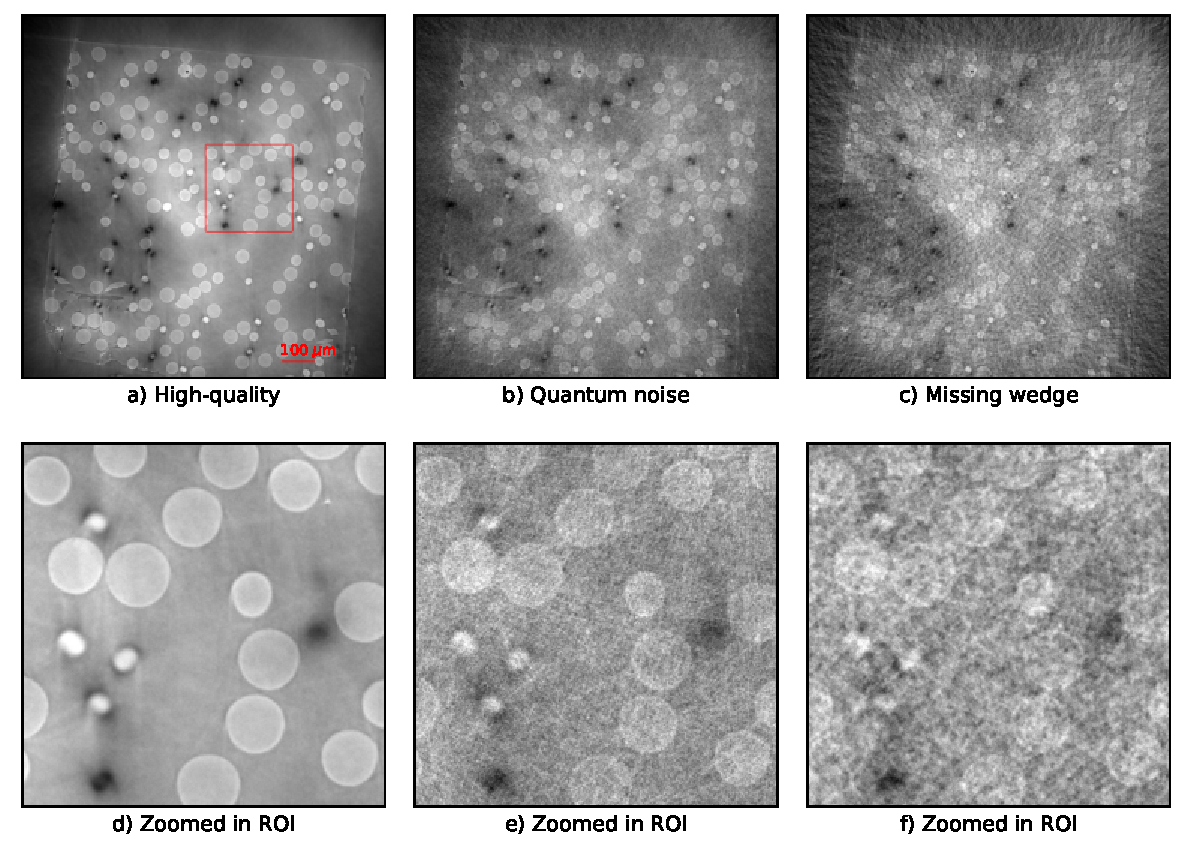
\includegraphics[width=.9\textwidth]{figures/noisecomparison.pdf}
    \caption[Reconstruction noise comparison]{Comparison of a high-quality reconstruction, a quantum noise reconstruction, and a missing wedge reconstruction. Images d), e), and f) are zoomed in \acrshort{roi}s of images a), b), and c) respectively. The \acrshort{roi} is marked in a). The quantum noise is simulated by applying Poisson noise to the sinogram, and the missing wedge problem is simulated by selecting a subsampling of every 32nd projection from the high-quality reconstruction. The images are of a central slice from the dataset tomo\_00058 \cite{datasetglassspheres} reconstructed using \acrshort{fbp} from TomoPy \cite{TomoBank}. }
    \label{fig:noisecomparison}
\end{figure}

\section{Imaging Method}
\todo[inline]{Keep this section?}
\subsection{Setup}
\missingfigure{Figure of generic CT setup, if section is staying. }

\section{Reconstruction}
After acquiring the attenuation coefficient projections, or sinograms, this data must be reconstructed into an image (of either 2D or 3D) of the object. The collection of a sinogram $P_\theta$ for projection angle $\theta$ is given by the Radon transform \cite{4307775,jimaging4110128}
\begin{equation}
    \label{eq:radontransform}
    P_\theta(u) = \iint f\left(x,y \right)\delta\left(x \cos \theta + y \sin \theta -u \right)dxdy,
\end{equation}
where $u$ is the position on the detector and $\delta$ is the Dirac delta function. In practice, because of computational and instrumental limitations, the projection data are acquired only for a limited number of projections $N_\theta$ as well as $N_d$ detector elements, and the imaged object is represented by a pixel grid of size $N \times N$. Thus, the acquired projection data is described by a vector $\bm{y} \in \mathbb{R}^{N_\theta \times N_d}$, the reconstructed image by a vector $\bm{x} \in \mathbb{R}^{N \times N}$, and the formation of the projection data can be stated as a linear system \cite{jimaging4110128}
\begin{equation}
    \label{eq:projectiondata}
    \bm{y} = \bm{A}\bm{x},
\end{equation}
where element $a_{ij} \in \mathbb{R}$ of $\bm{A} \in \mathbb{R}^{N_\theta N_d \times N^2}$ is equal to the contribution of image pixel $j$ to detector pixel $i$. This gives the tomographic reconstruction problem of recovering the unknown object $x$ from the acquired projection data $y$. It can be seen as performing the inverse Radon transform, which is known to be an ill-posed inverse problem \cite{KabanikhinIllVersed,GANrec}\footnote{Inverse problems are often ill-posed. An ill-posed problem is a problem that does not meet any one or more of the three conditions suggested by Jacques Hadamard: existence, uniqueness, and stability \cite{KabanikhinIllVersed}. The stability condition is most often violated. This means that its output is highly sensitive to small changes in the input (e.g. noise can drastically change the resulting output). }. 

Tomographic reconstruction algorithms are generally divided into two groups: direct reconstruction, and iterative reconstruction, however a third method using \acrshort{ml} has also shown some promise \cite{GANrec}.

\subsection{Direct Reconstruction}
Direct tomographic reconstruction algorithms are based on finding a continuous inversion formula of the continuous forward Radon transform, as given in \cref{eq:radontransform}, and discretizing the result \cite{jimaging4110128}. The most commonly used direct reconstruction algorithm is the \acrfull{fbp} algorithm, which can be written as \cite{jimaging4110128}
\begin{equation}
    \label{eq:fbp}
    \bm{x}_{FBP} = \bm{A}^T \bm{C}_h \bm{y},
\end{equation}
where $\bm{C}_h$ is a 1D convolution operation that convolves each detector row in $\bm{y}$ with a filter $\bm{h} \in \mathbb{R}^{N_d}$. The filter is typically some standard filter that can be used for any reconstruction (e.g. the Ram-Lak filter), and may include low-pass filtering to reduce high frequency noise in the reconstructed image \cite{681991}. It has also been shown that this filter can be learned by use of \acrshort{ml} (more specifically an \acrshort{ann}) to further improve the performance of \acrshort{fbp} \cite{6607157}. 

Direct algorithms, such as \acrshort{fbp}, have the advantage of most often being computationally efficient, as well as producing accurate results when enough projections are available \cite{jimaging4110128}. The issue with these techniques arises when a limited number of projections are available, as they are generally highly prone to noise leading to insufficient image quality for proper analysis \cite{jimaging4110128}. This is where the use for iterative reconstruction algorithms arises.

\todo[inline]{FDK? Same as FBP just for circular cone-beam projections instead of parallel \cite{Feldkamp:84}. }
\subsection{Iterative Reconstruction}
Iterative tomographic reconstruction algorithms are based on iteratively solving the linear system given in \cref{eq:projectiondata}. A common method used is to try and find reconstructed images that minimize the $l^2$-norm of the residual error (i.e. the difference between the acquired sinograms, and the Radon transform of the reconstructed image\footnote{Calculating the inverse Radon transform is an ill-posed problem and is challenging, however calculating the Radon transform itself is an easy task. }) as well as an additional term $g$ that penalizes images that do not confine to some prior knowledge or assumption of the imaged object. This process can be written as \cite{jimaging4110128}
\begin{equation}
    \label{eq:iterativesolution}
    \bm{x}_{iter} = \underset{\bm{x}}{\text{argmin}} \left|\left|\bm{y} - \bm{A}\bm{x}\right|\right|_2^2 + \lambda g(\bm{x}),
\end{equation}
where $\left|\left| \bm{\cdot} \right|\right|_2^2$ denotes the $l^2$-norm, and $\lambda$ is the relative weight of the prior knowledge penalty compared to the residual error. If a prior knowledge penalty that fits a reconstruction well is chosen, iterative reconstruction algorithms can produce significantly more accurate reconstructions than direct methods when reconstructing from limited data \cite{jimaging4110128}. If the chosen prior knowledge penalty does not fit well however, or if the weighting parameter $\lambda$ is poorly selected as it is a problem-dependent parameter, it may lead to poor quality reconstructions. 

A large drawback with iterative reconstruction is its (often) large computatinal cost. These types of reconstructions are slower, which may make it difficult to apply them to time-sensitive real-world tomographic data \cite{jimaging4110128}. Newer and more powerful computers can to some extent offset this downside to iterative reconstructions \cite{willemink2013iterative}. 

Because of these limitations and drawbacks, direct reconstruction algorithms are still often preferred in many fields \cite{Pan_2009}. 

\todo[inline]{PICCS \cite{piccs}}

\subsection{Other Methods}
In addition to direct and iterative reconstruction techniques, \acrshort{ml} has been used to make an iterative-like reconstruction algorithm \cite{GANrec}. One method, termed GANrec, is based on a \acrshort{gan} (which will be introduced in \cref{sec:ml:types:gan}) and is an \acrshort{ml} method that does not require training of the network before reconstruction, instead using the training process as the reconstruction process. 

It takes a given sinogram $\bm{y}$ and uses the generating network $G$ to create a candidate reconstructed image $\bm{x} = G(\bm{y})$, then creates the corresponding candidate sinogram $\hat{\bm{y}} = P(\bm{x})$, where $P$ is the Radon transform. The loss $L = \left|\left| y - \hat{y} \right|\right|$ is then the basis of training the network (i.e. reconstructing the image)\footnote{The actual loss used for training GANrec also includes an adversarial loss, which will be introduced in \cref{sec:ml:training:lossfunctions}, however it is omited in this description for the sake of simplicity. }.

The sinogram-to-reconstruction transformation cannot be done by a conventional \acrshort{cnn}-style network, however it has been shown that a single fully connected layer can perform this transformation \cite{PASCHALIS2004211}. The accuracy of the transformation can be improved by increasing the number of layers and neurons, however this is dependent on the available computational power \cite{GANrec}. Because of this limitation, the generating network in GANrec is a modified version of U-net \cite{unet}, which will be introduced in \cref{sec:ml:types:encoderdecoder}, with three fully connected layers at the start to perform this transform. 